\section{Model}

As we saw in the previous section, most preceding models suffer from one or more
of the following problems:
\begin{itemize}
	\item A rigidness that impedes variation and therefore creativity (the work
	of Chambers and Jurafsky learns very long and intricate schemata for its
	protagonist, making it gain coherence but losing flexibility)
	\item The starting scenario is the same every time (for
	example, in IN-TALE, there are very few possibilities for the story outcome,
	because the characters are the same for each story, and the ending is only
	dependent on the person playing the simulation).
	\item The story rules are made by hand (Gervás uses the story elements annotated
	by Propp, while in MEXICA the rules have been made by the creator of the
	program) or are lifted from knowledge bases not specifically designed for
	story generation (MAKEBELIEVE by Liu and Singh).
\end{itemize}
This section introduces the general problem of how to generate stories using
existing stories as a basis. Since
this problem is too complex to solve at once, it has to be divided into different sub-problems.
The work described in this paper aims to solve some of these problems (namely,
learn story rules from a set of annotated stories), but in
the next section some possible solutions for the unsolved sub-problems are also
given.

\subsection{Overall architecture}

Generating complete stories from a database of raw unannotated stories is a
complicated process, which has to be partitioned into multiple components.
The components of the general architecture which is assumed for this work is as follows:
\begin{itemize}
\item \textbf{A story database:} This would be the set of as many stories
as possible in a certain genre (for example, fairy tales), or possibly even
multiple genres, if the objective is to generate stories that are a hybrid
between genres. For now we assume these stories to be text, but in the future
this could possibly involve other types of media (film, videogames, etc.) as
well.
\item \textbf{A story synopsis database:} The stories in the story database have 
to be summarized in some way (for example \cite{salton1997automatic}). Another
option is to use human-made summaries, which exist for many stories already
(from Wikipedia or other internet sources, for example). In this way the story
is reduced to just the major plot elements, which should make rule extraction
easier (the story will be reduced to its bare essence, so there will be less 
long-term dependencies of story events).
\item \textbf{A database of logically represented stories:} There has to be some
way to transform the plot synopses into a logical representation (the rest of
this section will outline what this representation looks like). When this
structure is available, rules extracted from the stories can be made into a
queryable database.
\item \textbf{Generation of story synopses:} With the queryable database in place, a
planning algorithm can generate new story synopses, in such a way that they are
considered creative with respect to the existing database of synopses.
\item \textbf{Generation of full stories:} To make the stories enjoyable, the
plot synopses have to be transformed into full stories. This means expanding the
synopsis into a story with enjoyable prose. For other media, such as film or
videogames, creating images might be required too.
\end{itemize}
These components are visualized in a hierarchy in figure \ref{storypipeline}. In
this figure, there are three levels:
\begin{itemize}
\item The story level at the bottom, where the stories are in their full prose form.
\item The synopsis level in the middle, where the stories are in the form of a
human-readable synopsis.
\item The logic level at the top, where the stories are represented as a
sequence of states and actions, and where the rules are extracted from them.
\end{itemize}

\newcommand\myspacing{3.5}
\begin{figure}
	\begin{tikzpicture}[remember picture,
		outer/.style={draw=green,fill=green!20,thick,inner sep=10pt}
	]
		\node[outer,draw=green] (logic) at (0,0) {
			\begin{tikzpicture}
				\node[shape=rectangle,draw=black] (logicdb) at (2*\myspacing,0) {Database
				of logically represented stories};
			\end{tikzpicture}\\
		};
		\node[outer,draw=green] (synopsis) at (0,-3.5) {
			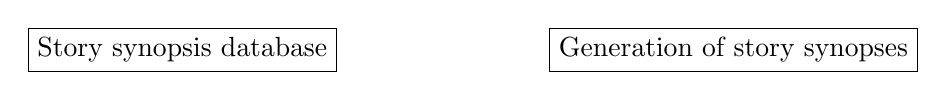
\begin{tikzpicture}
				\node[shape=rectangle,draw=black] (synopsisdb) at (\myspacing,0) {Story
				synopsis database};
				\node[shape=rectangle,draw=black] (synopsisgen) at (3*\myspacing,0)
				{Generation of story synopses};
			\end{tikzpicture}\\
		};
		\node[outer,draw=green] (story) at (0,-7) {
			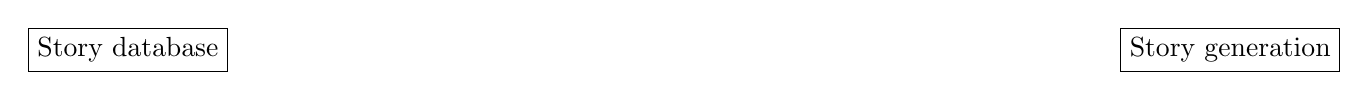
\begin{tikzpicture}
				\node[shape=rectangle,draw=black] (storydb) at (0,0) {Story
				database};
				\node[shape=rectangle,draw=black] (storygen) at (4*\myspacing,0) {Story
				generation};
			\end{tikzpicture}\\
		};
		\draw[-{Stealth[scale=3.0]}] (storydb) -- (synopsisdb);
		\draw[-{Stealth[scale=3.0]}](synopsisdb) -- (logicdb);
		\draw[-{Stealth[scale=3.0]}](logicdb) -- (synopsisgen);
		\draw[-{Stealth[scale=3.0]}](synopsisgen) -- (storygen);
	\end{tikzpicture}
	\caption{The story generation pipeline}
	\label{storypipeline}
\end{figure}

The focus of this thesis is twofold: the main contribution is a way to extract the rules found in a set of
logically represented stories, and represent them in such a way that a program can reason about
these rules in a creative way. This corresponds to the logic database component at the top
of figure \ref{storypipeline}, which details the assumed architecture. To do this, the story synopses have been
annotated manually to be able to focus on this part. However, the story
representation has been chosen in such a way that it could plausibly be extracted
in that form through natural language processing. 
This story annotation scheme is another contribution of this thesis. Its
simplicity makes it easy to annotate (and later, to be extracted automatically),
easy to visualize (which is important if this system is going to be used as a
co-creator with a human author) and easy to reason on (it is easy to find the
difference between different story states).
The overall approach of the work described in this thesis is as follows: the
stories are assumed to be annotated as a sequence of story states (represented
as graphs of characters, their wants and desires, and how these interact with
each other) and actions (simple sentences in natural language describing story
events). First, the action sentences are parsed to find the object, subject,
verb and dative (where applicable). Then, the preconditions of the actions (what
has to be true before this event can occur?) and the effects of the action (what
happens when this even takes place in the story?) are extracted, by looking at
the states prior and following the event. This information is then stored in a
database, which can be queried to obtain the likelihood of particular events.

\subsection{Story representation}

A basic story is represented by a series of states $s_i$ and actions $a_j$.
Each story starts in some initial state $s_0$, then one or more actions happen
($a_0, ..., a_j$), which lead to $s_1$. This is followed by one or more actions
again, which leads to $s_2$, and so on. This pattern continues until the final 
state of the story, which is where the story ends. This model is inspired by the
MEXICA model, although it is less constrained, since a state can be followed by
multiple actions instead of just one.

The story sequence is assumed to be represented temporally ($s_{i+1}$ occurs
after $s_i$). To represent events happening in parallel, stories can contain
stories themselves too. For example, in some stories, character A meets
character B at some place, and character B will tell character A about the
events that led character B to be at this particular place. Such a flashback
does not usually involve character A, and therefore can be considered a story within a
story. Another set of examples of stories where this construction would be
useful would be the stories of `One Thousand and One Nights' or `Canterbury Tales',
which are framing stories containing stories themselves. For the current algorithm, this construction does not
affect the rule extraction (the stories are read as separate stories), 
but for future deeper analysis this construction could be useful. If story
structure will also be learned from existing stories, this might be helpful to a
program that has to be able to generate flashbacks or framing stories.

\begin{figure}
	\begin{tikzpicture}[remember picture,
		outer/.style={draw=green,fill=green!20,thick,inner sep=10pt}
	]
		\node[outer,draw=green] (s1) at (0,0) {
			\begin{tikzpicture}
				\node[shape=rectangle,draw=black] (1p) at (0,0) {princess};
				\node[shape=rectangle,draw=black] (1pac) at (3.5,2) {princess\_abilities:companionship};
				\node[shape=rectangle,draw=black] (1pnb) at (3.5,-2) {princess\_needs:ball};
				\node[shape=rectangle,draw=black] (1pr1) at (7,0.75) {promise:1};
				\node[shape=rectangle,draw=black] (1pr2) at (7,-0.75) {promise:2};
				\node[shape=rectangle,draw=black] (1fab) at (10.5,2) {frog\_abilities:ball};
				\node[shape=rectangle,draw=black] (1fnc) at (10.5,-2) {frog\_needs:companionship};
				\node[shape=rectangle,draw=black] (1f) at (15,0) {frog};

				\draw[-] (1p) -- (1pac);
				\draw[-] (1p) -- (1pnb);
				\draw[-] (1pac) -- (1pr1) -- (1fnc);
				\draw[-] (1pnb) -- (1pr2) -- (1fab);
				\draw[-] (1fab) -- (1f);
				\draw[-] (1fnc) -- (1f);
			\end{tikzpicture}\\
			\textit{State 1}
		};
		\node[shape=rectangle,draw=black] (a1) at (0, -4) {the frog gets the ball};
		\node[outer,draw=green] at (0,-8) (s2) {
			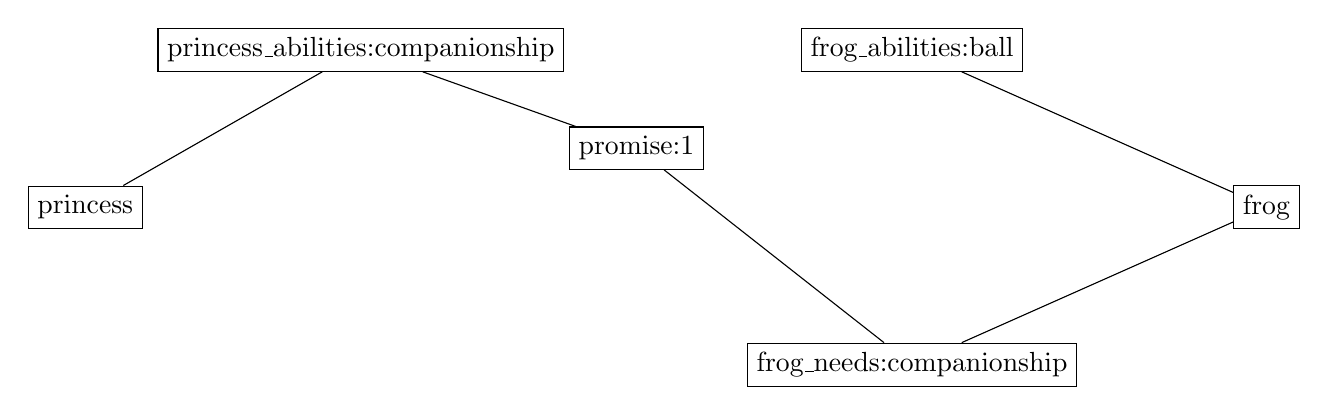
\begin{tikzpicture}
				\node[shape=rectangle,draw=black] (2p) at (0,0) {princess};
				\node[shape=rectangle,draw=black] (2pac) at (3.5,2) {princess\_abilities:companionship};
				\node[shape=rectangle,draw=black] (2pr1) at (7,0.75) {promise:1};
				\node[shape=rectangle,draw=black] (2fab) at (10.5,2) {frog\_abilities:ball};
				\node[shape=rectangle,draw=black] (2fnc) at (10.5,-2) {frog\_needs:companionship};
				\node[shape=rectangle,draw=black] (2f) at (15,0) {frog};

				\draw[-] (2p) -- (2pac);
				\draw[-] (2pac) -- (2pr1) -- (2fnc);
				\draw[-] (2fab) -- (2f);
				\draw[-] (2fnc) -- (2f);
			\end{tikzpicture}\\
			\textit{State 2}
		};
		\draw[-] (s1) -- (a1) -> (s2);
	\end{tikzpicture}
	\caption{Representation of a simple state-action-state transition.
	\textit{State 1}
	represents the part of ``The Frog Prince'' where the frog had promised to get
	the princess's golden ball from the bottom of a pond, in return for spending
	time with him (these promises are represented as relations between the
	relevant abilities and needs of the princess and the frog). There is one
	action, where the frog gets the ball for the princess, which leads to the
	altered state in \textit{State 2} (The princess does not need the ball
	anymore, and the promise has been fulfilled, which is why both nodes have
	been removed from the graph).}
	\label{storyrep}
\end{figure}

\subsubsection{States}

States are represented as a graph of filled with nodes representing currently
active characters, their abilities, and how these are connected with each other.
An example of two states can be seen in figure \ref{storyrep}.

\subsubsection{Actions}

Actions are represented as a short, natural language-like phrase (for example 
\texttt{``the frog gets the ball"}
or \texttt{``the frog promises the ball to the princess"}).
These sentences are parsed with the Python Natural Language Toolkit (NLTK)
\cite{BirdKleinLoper09}
to obtain the subject, verb and optionally the object and/or dative (which will be
referred to as $\texttt{subj}, \texttt{verb}, \texttt{obj}$ and $\texttt{dat}$,
respectively). For example "the frog gets the ball" would yield 
$\texttt{obj}=\textrm{``ball"}, \texttt{subj}=\textrm{"frog"},
\texttt{verb}=\textrm{``gets"}, \texttt{dat}=\textrm{``"} $. First the
sentences are tokenized (individual words are separated, comma's are separated
from the word they are attached to, etc.). Then NLTK assigns a
Part of Speech (P.O.S.) tag, denoting the lexical category that the word belongs
to. This takes care of the ambiguity found on the lexical level by looking at
the context in which the word appears (in the seconds example, ``promises" could
be a noun or a verb, but due to the context it is tagged as a verb). For the
experiments the P.O.S.-tagger recommended by the NLTK was used, which is a perceptron tagger
trained on the Penn Treebank dataset.

Then, the sentence is parsed using a simple tree-parser which uses a feature-based
grammar. This grammar contains rules to infer which word is the subject, which
word is the object, and so on. The rules in the grammar have the following form:
$$
\texttt{S}{[}\texttt{subj}=s, \texttt{verb}=v, \texttt{obj}=o, \texttt{dat}=d{]}
\Rightarrow
\texttt{NP}{[}\texttt{N}=s{]} \texttt{VP}{[}\texttt{V}=v, \texttt{N}=o,
\texttt{dat}=d{]}
$$
On the left hand side there is one non-terminal (in this case $\texttt{S}$), and
on the right hand side there is at least one terminal or non-terminal symbol
($\texttt{NP}$ and $\texttt{VP}$). The values for the variables are obtained in
a recursive fashion. This means that $s$, $v$ and $o$'s instantiation are dependent on the rules
chosen to expand the $\texttt{NP}$ and $\texttt{VP}$ nodes of the tree. After
enough node expansions a non-terminal will be expanded to a terminal, which will
instantiate the variables. This way we obtain values for $\texttt{subj}$ 
$\texttt{obj}$ $\texttt{verb}$ and $\texttt{dat}$. It is imporant to note again that
not all of these fields need to be instantiated. Most sentences don't have a
dative, and with intransitive verbs there is no object either (for example, the
sentence `John walks.' only has a subject (`John') and a verb (`walks')).
%TODO example of a parse?

\subsection{Rules}

\subsubsection{Rule representation}

Rule objects are similar in form to action objects. These are extracted from 
the stories by seeing how states are affected by a certain action.
They can be represented as a tuple of $(\texttt{action}, \texttt{obj}, \texttt{subj}, \texttt{dat},
\texttt{prec}, \texttt{eff})$.

Here, the verb denoting which action is taking place is stored in 
$\texttt{action}$
This is obtained from the parsed sentences' $\texttt{verb}$ field.
For example, ``promises'' is the action obtained from the
sentence \texttt{``the frog promises the ball to the princess''}, since
``promises'' is the verb of the sentence.

The dataset consists of fairy tales, which often contain certain stock 
characters (the king, the princess, the witch, etc.). These characters often
fullfill the same kind of role across fairy tales (the prince marries the
princess in many stories, for example).
This property is exploited by keeping track of a count of which agents
acted as objects, subjects, and datives in 
$\texttt{obj}, \texttt{subj}, \texttt{dat}$, respectively. That way, the program
could for example learn that the princess character rarely murders anyone, but
is more likely to marry someone (acting as the subject of the `marry' action) or
be married by someone (acting as the object of the `marry' action).

$\texttt{prec}$ represents the preconditions of the action in terms of what 
relations certain actors should have with each other (in other words, what has
to be true in the current story state before this action becomes possible?).
This is represented as a reduced subset of the action directly prior to the
action, only involving the characters involved in the action, their properties
and the relations between each character.
$\texttt{eff}$ represents the effects of the action (what
happens if this action is taken?). This is expressed in terms of either nodes in the
state graph appearing or dissappearing (these nodes can be characters, their
desires and abilities) or connections between nodes (representing the
connections between these entities) appearing or dissappearing.

For example, if $a = \texttt{"kill"}$, $\texttt{prec}$ might be 
$ \{\texttt{hates}(\texttt{subj}, \texttt{obj})\} $ (you have to hate someone 
before you kill them), and $\texttt{eff}$ would be ${\texttt{delete}(\texttt{obj})}$
(if you are killed, you are removed from the next state).
Note that both $\texttt{prec}$ and $\texttt{eff}$ are sets of conditions.
An action can have multiple prerequisites and multiple effects on the story state.

\subsubsection{Extracting rules}

Extracting the effect $\texttt{eff}$ of an action is the easiest. For now
actions are not assumed to have effects that do not become apparent immediately
(in other words, the action has an immediate effect on the next state, but no
lingering effects on the states after that).
Therefore it is enough to see what the difference is between the state before
and the state after the action. The different concepts that are tracked are the
nodes in the graph that appear and disappear in the new state, and the
connections that appear and dissappear in the new state.

However, because multiple actions can appear between states it is difficult to
discern which actions affects what parts of the network. 
Therefore, for each action, the algorithm only looks at the actors involved in 
the action ($\texttt{obj}, \texttt{subj}, \texttt{dat}$), and the nodes
connected to them directly (these nodes are assumed to be either desires or
abilities of the characters). This keeps the preconditions managable too, since
they don't just include the whole state difference, but only the relevant parts
for the action. Of course this assumption breaks down if a lot of actions
between two states
involve the same actor (making it unclear what action had what effect), but this pruning of possible actors does already reduce
the ambiguity in a meaningful way.

At first the program only looked at the characters themselves, but since the
interesting relations were mostly between the desires and abilities of the
characters, and not the characters themselves (for example, in figure
\ref{storyrep} there is no direct relation between the princess and frog nodes,
but their abilities and desires are linked to promises), this did not pick up the more
interesting preconditions and effects of each action.

So, in figure \ref{storyrep} the frog node and the nodes containing the word
"ball" ("frog\_abilities:ball" and "princess\_needs:ball") are considered, as
well as their immediate neighbor nodes and the connections to them (in effect,
the whole first state without the princess node).

Similar to effects, for the preconditions $\texttt{prec}$ the state immediately prior to the action
is assumed to have all the
necessary information for the action in it (it is not necessary to look at the 
preceding states, since they offer no additional information). Therefore all
information in the previous state is assumed to be a part of the precondition.
However, this is reduced like the preconditions to only the actors involved in
the action, and the nodes directly connected to them.

Another thing that is also stored is in which story a particular occurence of a
rule was found. This can later be helpful if the program is used as a tool for
story analysis, but could also be used to guide the creation process of a
generation algorithm, by introducing a bias for certain stories if so desired.
This bias would be helpful if the program would be allowed to train on stories
it generated itself, giving preference to human-created stories, since they are
known to be well-constructed.

\subsubsection{Querying the rules}

All extracted actions are stored together in a database (in the current
implementation this is a Python dictionary, with the actions as keys and the
rest of the information stored in an object as a value). This database can be
queried for the probabilities of certain actions: 
$$p(a) = \frac{\it{Count}(a)}{\sum_{x \in A}\it{Count}(x)}$$
Here $a$ is the action and $A$ is the set of all seen actions.
We can also query the database in a conditional manner (for
example, if we want to find some action for the princess to do in the story, we
can simply query the probability of different actions, given that the princess
is the subject of the action:
$$p(a \mid a_{\texttt{subj}}=\texttt{"princess"}) = 
\frac{\it{Count}(a \land a_{\texttt{subj}}=\texttt{"princess"})}{\it{Count}(a)}$$
These probabilities can be used by a planning algorithm to generate stories in a
creative manner. In the introduction of this paper, we noted that for artistic
creativity, in this case story generation, we have to generate stories
that are both novel but are also comprehensible. With the action probabilities,
we have a metric of how plausible certain actions are, so a planning algorithm
could choose the next action based on how plausible the story is. If the story
is following the existing stories too much (the probability of the
generated story becomes too high), it can choose an action with a
low probability in an attempt to make the story more creative. But if the story becomes too
unpredictable (the probability of the story becomes too low), the program might
choose an action with a high probability to try to balance things out. However, finding
which exact values to use for the upper and lower boundaries for this algorithm
would require more annotated stories to do a proper analysis, and is therefore
outside the scope of this thesis.
